\subsection{Документ формирование заказа поставщикам}
\subsubsection{Тестовая версия документа}
\begin{itemize}	
	\item Для формирования заказа поставщикам создана тестовая версия документа.
		\sidenote[-2ex][]{Принимаются замечания и пожелания}.
	\item Документ "<Формирование заказов поставщикам"> включен в интерфейс в подсистему "<Закупки">. \par После открытия документа необходимо заполнить реквизиты требуемые для работы. 	
	\begin{figure}[H]
		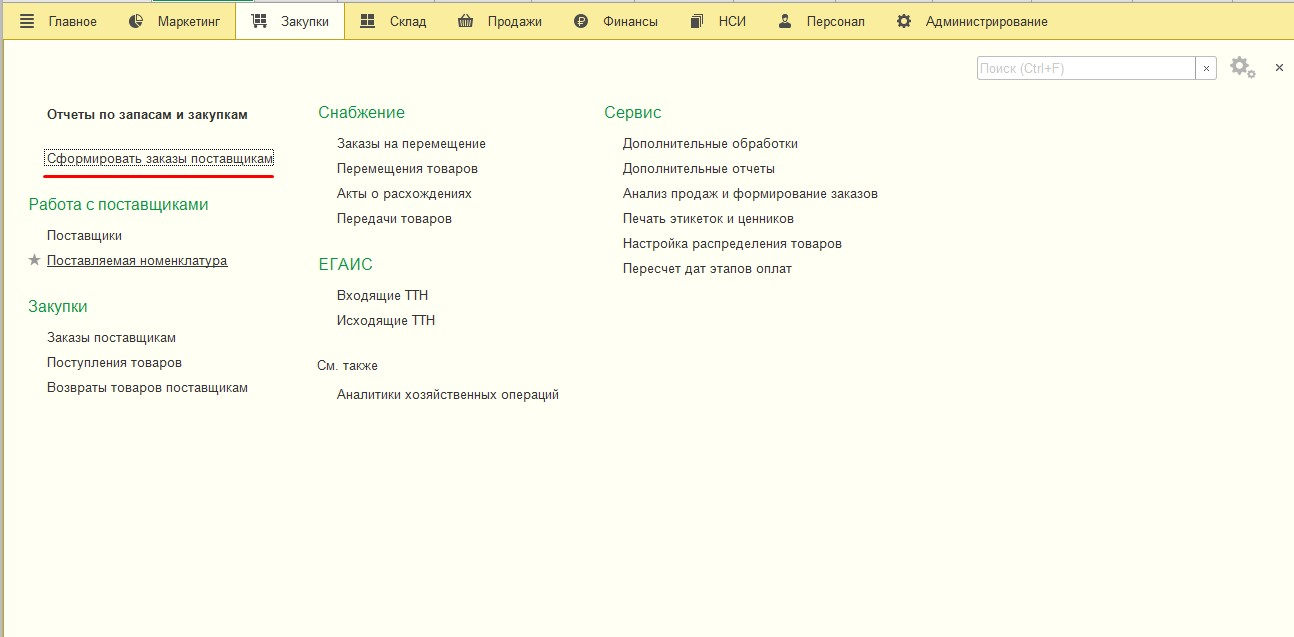
\includegraphics[width=0.90\textwidth]{94.jpg}
		\caption{Документ "<Формирование заказов поставщикам">.}
		\label{ris:94.jpg}
	\end{figure}

	\begin{enumerate}[I]
		\item "<Дата"> - Заполняется автоматически, это дата документа. Дата когда формируем заказы
		\item "<Период для анализа">  "<С:">  и "<По:">- Месяц, за который будет произведен анализ продаж.\par
		Необходимо указывать предшествующий расчетному \textbf{календарный} месяц.		
		\sidenote[-2ex][]{\textbf{Внимание!}}.
		\begin{figure}[H]
			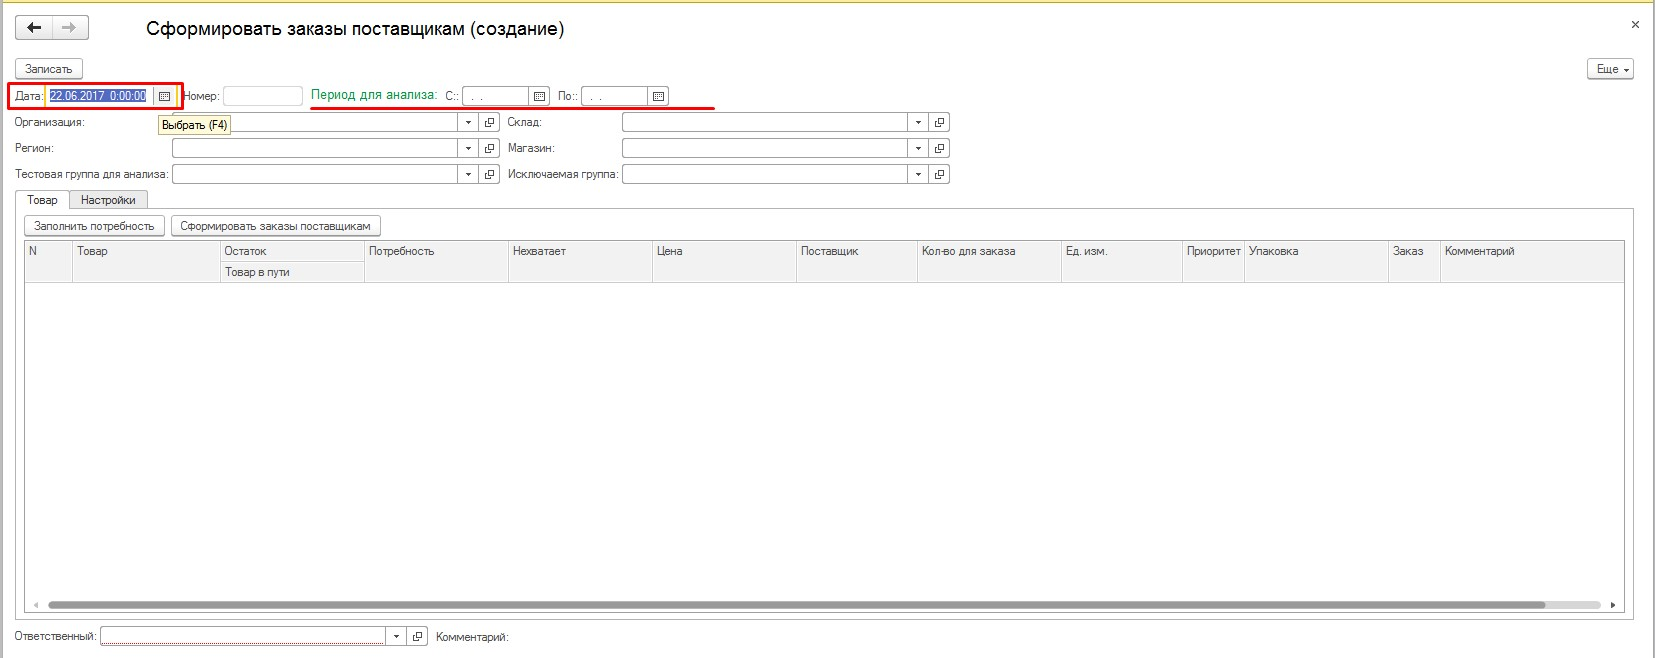
\includegraphics[width=0.99\textwidth]{90.jpg}
			\caption{Заполнение периодов.}
			\label{ris:90.jpg}
		\end{figure}
		\item "<Исключаемая Группа"> - Группа номенклатуры, которая не должна попадать в анализ и заказы
		\item "<Регион"> - Регион по которому выполняем анализ.		
		\item "<Тестовая группа для анализа"> - Группа номенклатуры включаемая в анализ (возможно тестовый реквизит)
		\item "<Магазин"> - Магазин, в котором формируют заказ
		\item "<Склад"> - Склад для заказа.		
		\item "<Организация"> - Организация
		\begin{figure}[H]
			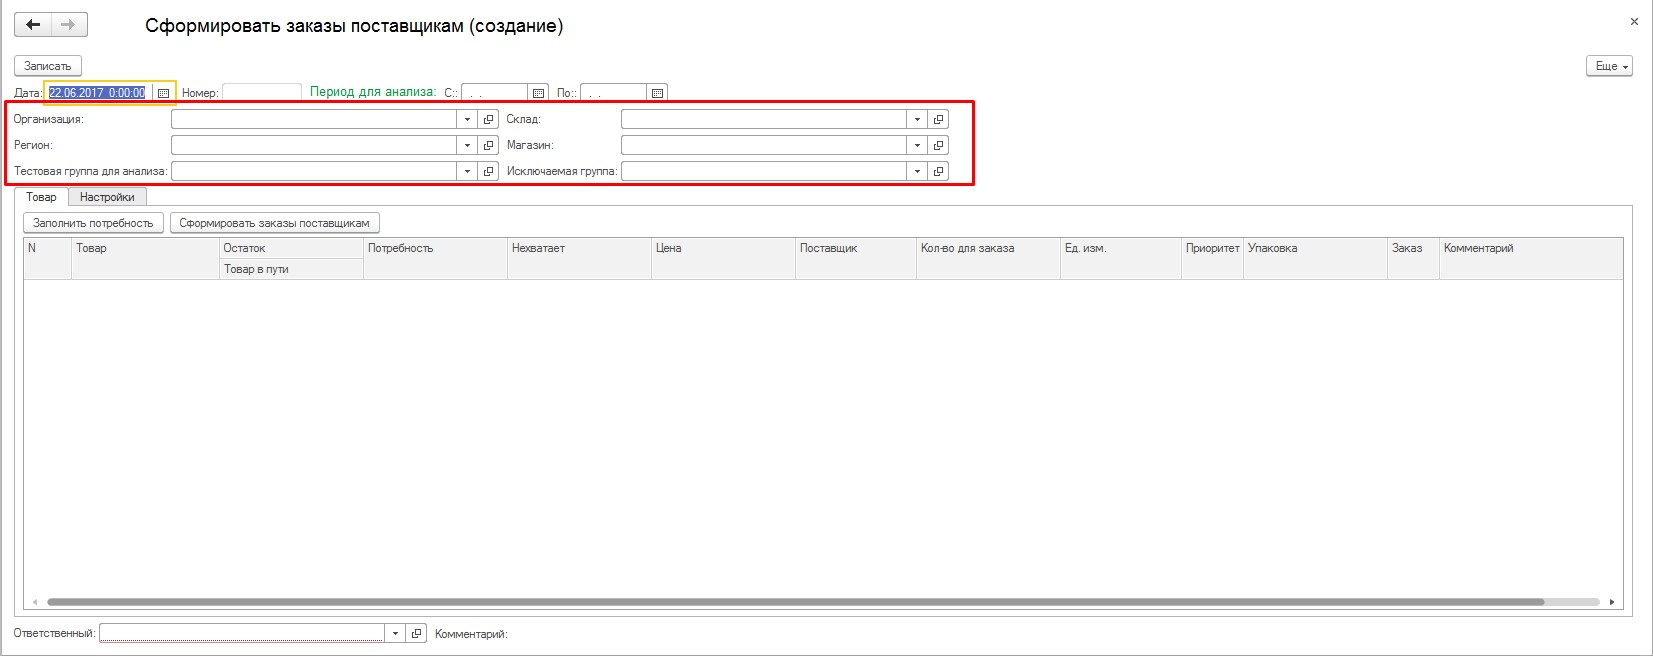
\includegraphics[width=0.99\textwidth]{91.jpg}
			\caption{Отбор номенклатуры и магазинов.}
			\label{ris:91.jpg}
		\end{figure}		
	\end{enumerate}
	\item После того, как все реквизиты заполнены, по нажатию кнопки \keys{Заполнить потребность} происходит заполнение табличной части обработки с предварительными данными для формирования заказов. 		
	\begin{figure}[H]
		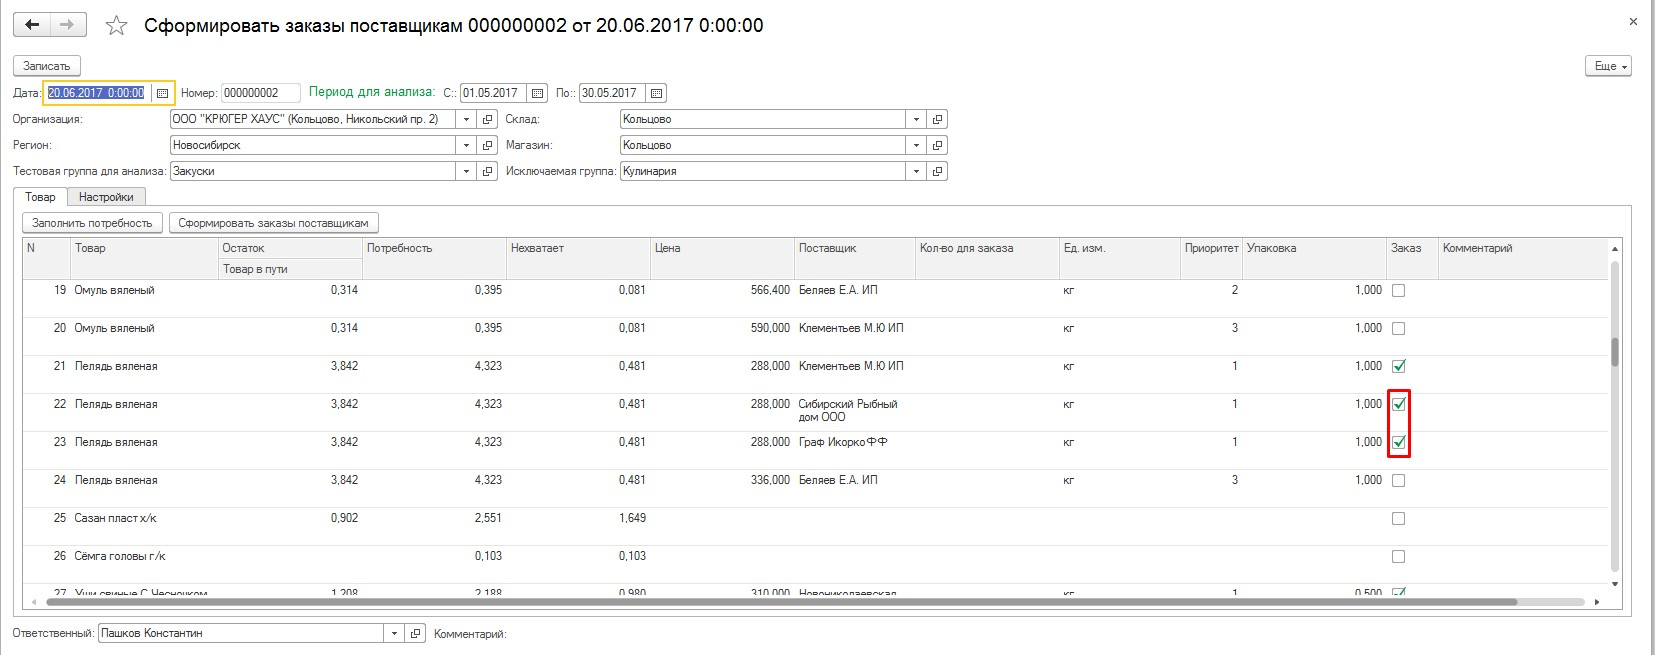
\includegraphics[width=0.99\textwidth]{93.jpg}
		\caption{Таблица для заказов.}
		\label{ris:93.jpg}
	\end{figure}		
	\item В колонке заказ проставлены "<галочки"> для рекомендуемого заказа, (на данном этапе алгоритм расчета такой: сначала среди поставщиков выбирается минимальная цена, а для позиций с одинаковой ценой, строка с минимальным числом приоритета у поставщика, если есть несколько строк с одинаковой ценой и приоритетом, то "<галочки"> проставляются для всех подобных строк) ответственное лицо может их  снимать, добавлять.\par  После того, как отмечены нужные позиции, для формирования документов "<Заказ поставщику"> нужно нажать кнопку \keys{Сформировать заказы поставщикам}.\par
	\item	На странице "<Настройка"> Можно указать учитывать или нет при расчете потребности товара возвраты покупателя и заказанные, но еще не полученные товары. Если выбрано "<Учитывать возвраты">, то в обязательном порядке необходимо указать аналитику хозяйственной операции по которой будет производится отбор документов возврата (если не указать, то документы возврата учтены не будут). В общем случае это "<Возврат от покупателя">
	Учет возврата от покупателя будет уменьшать "<Потребность"> товара за текущий анализируемый период.\par
	При включенном учете недополученных заказов количество товара в заказе будет по подать в колонку "<Товар в пути"> и соответственно будет уменьшено количество товара в колонке "<Нехватает">.
	
		\begin{figure}[H]
		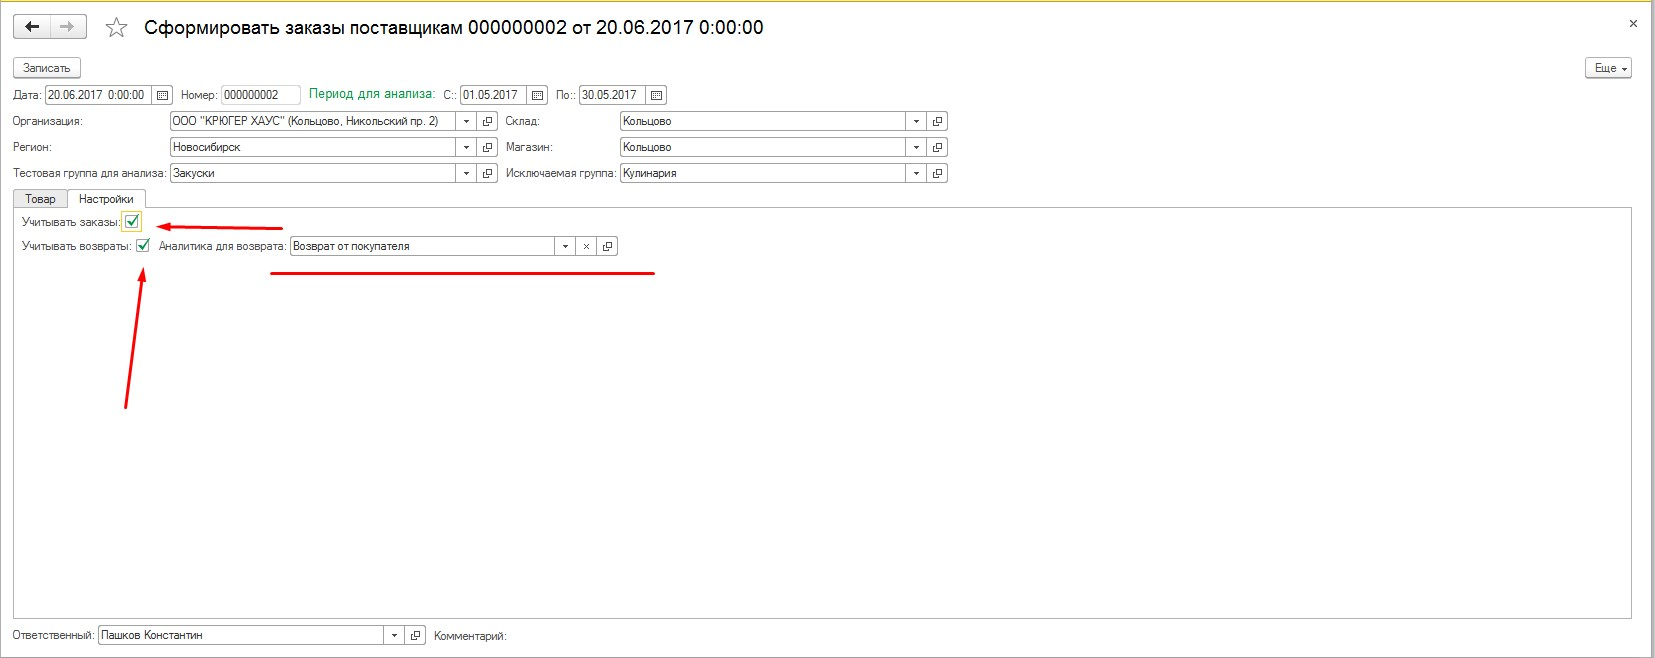
\includegraphics[width=0.99\textwidth]{92.jpg}
		\caption{Настройка.}
		\label{ris:92.jpg}
	\end{figure}		
	
	\item Сформированные заказы можно увидеть в журнале документов "<Заказ поставщику">. 

\end{itemize}